Tous les codes de cette leçon sont dans le projet "matrices". En plus des codes demandés, plusieurs choses ont été imlémentées. D'une part une interface "Matrix" qui représente une matrice générique et une classe "Utilities" qui implémente plusieurs opérations sur les matrices (addition, affichage, ...).

\begin{figure}[H]
	\caption{\label{struc} Diagramme de la structure du projet "matrices"}
	\centering
	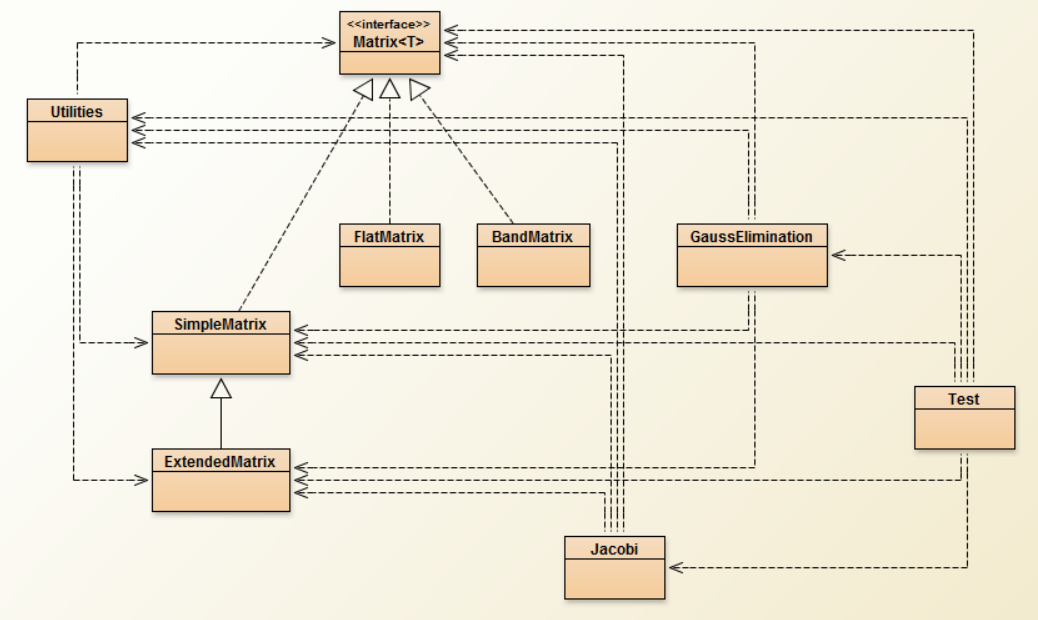
\includegraphics[scale = 0.6]{2_structure.png}
\end{figure}

Tous ce code est expérimental et ne peut pas être utilisé tel quel dans un projet. En effet, ils risquent de générer des erreurs, par exemple parce qu'ils ne vérifient jamais si les données sont correctement formatées. Le but est avant tout de se concentrer sur les algos et leur fonctionnement.

\subsection{Question 1}
\code{matrices}{FlatMatrix.java}

\subsection{Question 2}

// TO DO

\subsection{Question 3}

\subsubsection{Java representation of a band matrix}
\code{matrices}{BandMatrix.java}

\subsubsection{Multiplication by a band matrix}
\codelocation{matrices}{Utilities.java}
\begin{lstlisting}
public static Matrix multiplyByBand(Matrix base, Matrix band) {
    SimpleMatrix ret = new SimpleMatrix(base.getHeight(), base.getWidth());
    for (int i = 0; i < base.getHeight(); i++) {
        for (int j = 0; j < base.getWidth(); j++) {
            double pos = (double) base.get(i, j-1)* (double) band.get(j-1, j) + (double) base.get(i, j)*(double) band.get(j, j);
            ret.set(pos, i, j);
        }
    }
    return ret;
}
\end{lstlisting}